\documentclass[11pt]{article}

\usepackage[margin=1in]{geometry}
\usepackage{mathptmx}
\usepackage[T1]{fontenc}
\usepackage{amsmath,amssymb,amsthm}
\usepackage{graphicx}
\usepackage{booktabs}
\usepackage{caption}
\usepackage{subcaption}
\usepackage[colorlinks=true,linkcolor=blue!50!black,citecolor=blue!50!black,urlcolor=blue!50!black]{hyperref}
\usepackage[round,authoryear]{natbib}
\usepackage{doi}
\usepackage{xcolor}
\usepackage[section]{placeins}
\usepackage{enumitem}
\usepackage{titlesec}
\usepackage{abstract}

\graphicspath{{figures/}}

\titleformat{\section}{\normalfont\large\bfseries}{\thesection}{1em}{}
\titleformat{\subsection}{\normalfont\bfseries}{\thesubsection}{1em}{}

\newtheorem{proposition}{Proposition}
\newtheorem{assumption}{Assumption}

\newcommand{\R}{\mathbb{R}}
\newcommand{\E}{\mathbb{E}}
\newcommand{\Dir}{\mathrm{Dirichlet}}
\newcommand{\GOAL}{\textsc{Goal}}
\newcommand{\NOGOAL}{\textsc{Shot}_{\text{no goal}}}
\newcommand{\TURN}{\textsc{Turnover}}

\title{\bfseries Possession-Clock Markov Decision Processes for Football:\\
A Bayesian Hierarchical Framework for Simulating and\\ Evaluating Tactical Policy}

\author{
Waltzing Analytics\\
\small \texttt{Ecuador 2026 Liga Pro Research Notes}
}
\date{\today}

\begin{document}
\maketitle

\begin{abstract}
We model football possessions as episodes from team-specific nonstationary Markov decision processes (MDPs) with transition probabilities that depend on the \emph{possession clock} -- the time elapsed since a team won the ball -- adapting a modeling framework originally developed for shot-clock-dependent basketball play simulation. Bayesian hierarchical models parametrize these transition probabilities, pooling across lineups, opponents, and the season via a three-level (league, team, lineup) Dirichlet-Multinomial cascade. To keep multi-lineup, season-long simulation tractable, we combine lineup-specific MDPs into a single team-average MDP using a transition-weighting scheme: the team-average process is constructed so that its expected transition count for any state pair equals the exposure-weighted sum of the expected counts of the separate lineup-specific MDPs. We solve the resulting nonstationary MDPs for their value functions by value iteration, and use them to drive a Monte Carlo possession simulator in which posterior parameter uncertainty is propagated into simulated outcomes. Fitting the model to a full season of Ecuadorian Liga Pro event data (136 matches, 16 teams, 37{,}075 possession episodes), we find that turnover risk peaks in the first five seconds after winning the ball rather than rising monotonically as the possession clock runs out, that value is a smooth, monotonically increasing function of proximity to goal peaking inside the penalty area, and that teams occupy a comparably-sized region of forward/sideways/backward build-up styles rather than clustering near any one extreme. We further show that a naive comparison of two independently-simulated policies is statistically unreliable for rare-event outcomes such as goals -- a paired-simulation design that shares the dynamics draw across both policies is required to obtain a stable estimate of a policy change's effect -- and use the corrected estimator to rank all 16 league teams by their simulated benefit from a more direct style of play. We close with a discussion of the game-theoretic limits of fixed-dynamics counterfactual simulation.
\end{abstract}

\section{Introduction}
\label{sec:intro}

Possession-based sports share a common structural feature: within a possession, a team makes a sequence of decisions that produce a sequence of on-ball states -- where the ball is, how much time remains under some clock -- until the possession ends in a score, a loss of the ball, or a stoppage. The basketball analytics literature has formalized this as a team-specific, shot-clock-dependent Markov decision process (MDP): the state captures ball location and shot-clock value, the action captures the decision made with the ball, and the transition captures both the outcome of that decision and the resulting next state. Because basketball's 24-second shot clock imposes a hard, common, exogenous deadline, it is a natural driver of nonstationarity: teams behave differently with 20 seconds left on the shot clock than with three.

Football has no shot clock, but it has a close analogue: the \emph{possession clock}, the number of seconds a team has controlled the ball since the turnover, restart, or recovery that started the current possession. Empirically, the character of a possession changes with this clock in ways that echo the basketball shot clock, although not always in the direction a naive analogy would predict (Section~\ref{sec:results-hazard}). Early in a possession, teams probe and circulate the ball; as the clock runs on, defensive shape has more time to organize around the ball. Unlike the shot clock, the possession clock is unbounded and endogenous -- it resets on every turnover rather than counting down to a forced action -- but it plays the same statistical role: it is the variable that makes the transition probabilities \emph{nonstationary within an episode}, and the variable a hierarchical model must condition on to avoid pooling together possessions that are behaviorally very different.

This paper adapts the possession-MDP framework to football possessions, using three structural ideas: (i) team- and lineup-specific nonstationary MDPs indexed by the possession clock in place of the shot clock; (ii) Bayesian hierarchical parametrization of the transition probabilities, pooling across lineups, the roster's turnover through substitutions, and the season; and (iii) a transition-weighting scheme that combines lineup-specific MDPs into a single team-average MDP whose expected transition counts equal the exposure-weighted sum of the lineup-specific expected counts, making season-long, multi-lineup simulation computationally tractable without discarding the lineup structure in the data. We then solve the fitted MDPs for their value functions, build a possession simulator from them, propagate posterior uncertainty into simulated outcomes, and use the simulator to compare on-policy and altered-policy season simulations. We fit this model to a full season of Ecuadorian Liga Pro event data and report both the fitted model's qualitative empirical findings and the results of the policy counterfactual.

\section{Related Work}
\label{sec:related}

Possession-outcome modeling in basketball has an established literature; \citet{cervone2016multiresolution} model basketball possessions as a multiresolution stochastic process to produce a point-value estimate for every moment of a possession, from which league-wide and player-specific value can be derived. The present work follows the same broad ambition -- turning a possession into a stochastic process whose value can be solved for and whose policy can be perturbed -- but adapts it to a football-specific state representation (pitch zone crossed with possession clock, rather than continuous player-tracking coordinates), and to football's characteristic data constraints: far fewer possessions are observed per team per season than in basketball, motivating the three-level Bayesian hierarchy and the team-average transition-weighting scheme that are the technical core of this paper.

\section{Data}
\label{sec:data}

We use Opta/Stats Perform F24-style event data from the 2026 Ecuadorian Liga Pro season: 136 matches across 16 teams, covering every on-ball event (passes, take-ons, tackles, interceptions, clearances, aerials, ball recoveries, shots, goals, substitutions, and starting lineups) with pitch coordinates, qualifiers, and timestamps. Team lineups at every point in a match are reconstructed from starting-XI and substitution events. Possession episodes are segmented directly from the chronological event stream: a new episode begins whenever ball control changes to a different team (a successful pass, take-on, aerial win, or recovery), and ends in a goal, a saved or missed shot, a failed pass or take-on, a defensive interception, tackle, clearance, or foul conceded, or the end of a playing period. Across the season this yields 37{,}075 possession episodes. Own-goal events (identified by the Opta ``own goal'' qualifier) are excluded from the shot/goal stream, since they are otherwise misattributed to the benefiting team as a shot taken from wherever the defensive touch occurred -- typically deep in that team's own defensive third -- which would corrupt both the fitted transition probabilities and the value function described in Section~\ref{sec:valuefunction}.

\section{Football Possessions as Episodes of a Nonstationary MDP}
\label{sec:mdp}

\subsection{Episodes}
An \emph{episode} is a single team's possession: it begins the moment that team gains controlled use of the ball and ends when the ball is lost, a shot is taken, or play is stopped in a way that hands the opponent the restart.

\subsection{State space}
The state at any point within an episode is
\begin{equation}
s = (z, c), \qquad z \in \{1,\dots,Z\}, \quad c \in \{1,\dots,C\},
\end{equation}
where $z$ is the \emph{pitch zone} the ball occupies, taken from a $6\times 4$ grid over the attacking half-space of the pitch (length $\times$ width, with $x=100$ always meaning ``closest to the opponent's goal'' in the possessing team's attacking direction), and $c$ is the \emph{possession-clock bucket}, a discretization of seconds elapsed since the possession began into five bins: $[0,5)$, $[5,10)$, $[10,15)$, $[15,25)$, and $[25,\infty)$ seconds. Two absorbing outcome states close every episode: $\GOAL$ and $\TURN$; a non-scoring shot ($\NOGOAL$) is tracked as a third, separate terminal outcome for efficiency reporting even though it plays the same absorbing role as a turnover from the MDP's point of view.

\subsection{Action space}
At each non-terminal state the team on the ball chooses an action
\begin{equation}
a \in \{\text{advance}, \text{sideways}, \text{back}, \text{cross}, \text{shot}\},
\end{equation}
capturing the \emph{attempted} decision -- the direction and type of the pass, carry, or shot attempted -- independent of whether it succeeds. This mirrors the basketball MDP's separation of a decision (e.g. ``attempt a three-pointer'') from its outcome (make, miss, or turnover): the outcome of an ``advance'' decision -- successful progression, an intercepted or misplaced pass, a foul won -- is captured by the transition, not the action label.

\subsection{Transitions and nonstationarity}
Given a state-action pair $(s,a)$ with $s=(z,c)$, the transition distribution
\begin{equation}
P(s' \mid s, a), \qquad s' \in \{1,\dots,Z\}\times\{1,\dots,C\} \cup \{\GOAL, \NOGOAL, \TURN\},
\end{equation}
gives the probability of each destination zone (with the clock advanced to the next bucket, or capped at the final bucket), or of the possession ending. The distribution is explicitly allowed to depend on $c$: this is the direct analogue of shot-clock-dependent transition probabilities in the basketball model, and Section~\ref{sec:results-hazard} shows the dependence is real and, in one respect, the opposite of what a naive shot-clock analogy would predict.

\subsection{The Markov property}
\label{sec:markov}
The defining assumption of the model is that $P(s' \mid s, a)$ depends only on the current state and action, not on the sequence of states and actions that preceded it: a pass attempted from ``final third, central, 0--5s'' is modeled identically whether the team arrived there via a 25-pass build-up or a single long ball. This is a simplification rather than a claim about football itself -- it is precisely what makes a season of possessions tractable to fit as a single model, and Section~\ref{sec:limitations} returns to where it strains, e.g. its inability to distinguish a fatigued team from a fresh one occupying the same state.

\section{Bayesian Hierarchical Parametrization}
\label{sec:hierarchy}

Football produces far fewer possessions per team per season than basketball produces shot-clock states, and the possession-clock $\times$ zone $\times$ action state space is large relative to the data available for any one lineup. Naively estimating $P(s' \mid s,a)$ separately for each lineup a team fields over a season would leave most cells with a handful of observations or none. We borrow strength using a three-level Bayesian hierarchy with a Dirichlet--Multinomial conjugate structure at each level:
\begin{align}
\alpha^{\text{league}}(s,a) &= \kappa_{\text{league}} \cdot \bar p^{\,0}(s,a) + n^{\text{league}}(s,a), \\
\alpha^{\text{team}}_T(s,a) &= \kappa_{\text{team}} \cdot \bar p^{\,\text{league}}(s,a) + n^{\text{team}}_T(s,a), \\
\alpha^{\text{lineup}}_{T,L}(s,a) &= \kappa_{\text{lineup}} \cdot \bar p^{\,\text{team}}_T(s,a) + n^{\text{lineup}}_{T,L}(s,a),
\end{align}
where $\bar p^{\,\ell}(s,a)$ denotes the posterior-mean outcome distribution at level $\ell$, $\bar p^{\,0}$ is a base rate (uniform over the outcomes empirically observed anywhere in the league for that cell), $\kappa_{\text{league}}, \kappa_{\text{team}}, \kappa_{\text{lineup}}$ are concentration hyperparameters controlling how strongly each level is pulled toward its parent, and $n^{\,\ell}(s,a)$ is the vector of observed transition counts at that level. A sparsely visited $(s,a)$ cell for a given lineup is shrunk heavily toward that team's overall tendency in the same zone/clock state; a frequently visited cell for a settled first-choice lineup is dominated by its own data. We pool across the same hierarchy for the action-choice policy $\pi(a \mid s)$, using a two-level (league $\to$ team) cascade, since altered-policy simulation (Section~\ref{sec:policy-sim}) operates at the team level.

Counts are further weighted by an exponential recency factor $w_k = \rho^{(K-k)/7}$ for a match played $k$ weeks before the most recent matchday $K$ ($\rho = 0.98$), so that current transition estimates reflect a team's most recent tactical identity more than its early-season form while still using the full season's data.

\section{From Lineup MDPs to a Team-Average MDP}
\label{sec:teamavg}

A team fields many distinct lineups over a season, and each lineup induces its own MDP with its own transition probabilities $P_L(s' \mid s, a)$. Simulating a season faithfully would require carrying every lineup's MDP forward separately -- exact, but computationally unwieldy once posterior uncertainty and multi-episode simulation are layered on top. We instead define a single \emph{team-average MDP} per team, constructed so that it reproduces, in expectation, the transition behavior actually generated by the mix of lineups the team used.

Let $w_L$ be the team's \emph{lineup exposure weight} -- the share of the team's total possession volume played by lineup $L$ -- and let $n_L(s,a)$ be the observed number of times lineup $L$ visited $(s,a)$. Define the team-average transition distribution as the exposure- and volume-weighted mixture of the lineup-specific posterior means:
\begin{equation}
P_T(s' \mid s,a) = \frac{\sum_L w_L \, n_L(s,a) \, P_L(s' \mid s,a)}{\sum_L w_L \, n_L(s,a)}.
\label{eq:teamavg}
\end{equation}

\begin{proposition}[Expected-count consistency]
Let $N$ be the total number of visits to $(s,a)$ across a team's lineups, allocated across lineups in proportion to $w_L\, n_L(s,a)$. Then the team-average process's expected transition count for the state pair $(s,a,s')$ equals the exposure-weighted sum of the expected counts of the separate lineup-specific MDPs:
\begin{equation}
N \cdot P_T(s' \mid s,a) = \sum_L w_L\, n_L(s,a)\, P_L(s' \mid s,a) \cdot \frac{N}{\sum_L w_L\, n_L(s,a)}.
\end{equation}
\end{proposition}
\begin{proof}
Immediate from substituting Equation~\eqref{eq:teamavg} and canceling the shared normalizer $\sum_L w_L\, n_L(s,a)$.
\end{proof}

This is stronger than pooling raw transition counts across lineups before normalizing, which would overweight whichever lineup happened to visit $(s,a)$ most often, independent of how much of the team's overall play that lineup represents; weighting by $w_L$ first ties the team-average process to how the manager actually used the squad. In practice $P_T$ is computed from the \emph{posterior} lineup distributions (Section~\ref{sec:hierarchy}), so that thin lineup samples are shrunk before being folded into the team average, expressed as a synthetic Dirichlet parameter vector (mean matched to the weighted mixture, total concentration matched to the combined lineup evidence, floored at a minimum of 3 pseudo-observations) so that the simulator (Section~\ref{sec:simulator}) can draw posterior samples from the team-average MDP exactly as it would from any other level of the hierarchy.

\section{The Value Function}
\label{sec:valuefunction}

Because every state points to other states or to a terminal outcome, the fitted MDP can be solved for more than its next-step transition probabilities: for any state $s$, the \emph{value} $V(s)$ is the probability that continuing to play out a possession from $s$, under the team's fitted policy and dynamics, eventually ends in a goal. This is the fixed point of the Bellman equation
\begin{equation}
V(s) = \sum_{a} \pi(a \mid s) \sum_{s'} P(s' \mid s,a)\, r(s'), \qquad r(s') = \begin{cases} 1 & s' = \GOAL \\ 0 & s' \in \{\NOGOAL, \TURN\} \\ V(s') & \text{otherwise,} \end{cases}
\label{eq:bellman}
\end{equation}
solved by value iteration: initializing $V \equiv 0$ and repeatedly substituting the current estimate of $V$ into the right-hand side of Equation~\eqref{eq:bellman} until convergence (150 sweeps is more than sufficient given the per-step probability of reaching an absorbing state).

Figure~\ref{fig:valuefunction} shows the solved value function for Independiente del Valle, faceted by possession-clock bucket. Value rises smoothly and monotonically with proximity to the opponent's goal in every clock bucket, from under 1\% deep in the team's own defensive third to 12--19\% inside the penalty area -- an order-of-magnitude gradient, and exactly the shape a value function fit to a coherent possession model should have. This also serves as a useful diagnostic: an early, uncorrected version of this computation (in which own-goal events were still being attributed to the scoring team as their own converted shot, and in which pitch-heatmap labels were placed without accounting for the plotting library's vertical-pitch coordinate flip) instead showed defensive-third zones as more valuable than the penalty area, which is the kind of qualitatively implausible result that a value-function sanity check is well suited to catch.

\begin{figure}[htbp]
\centering
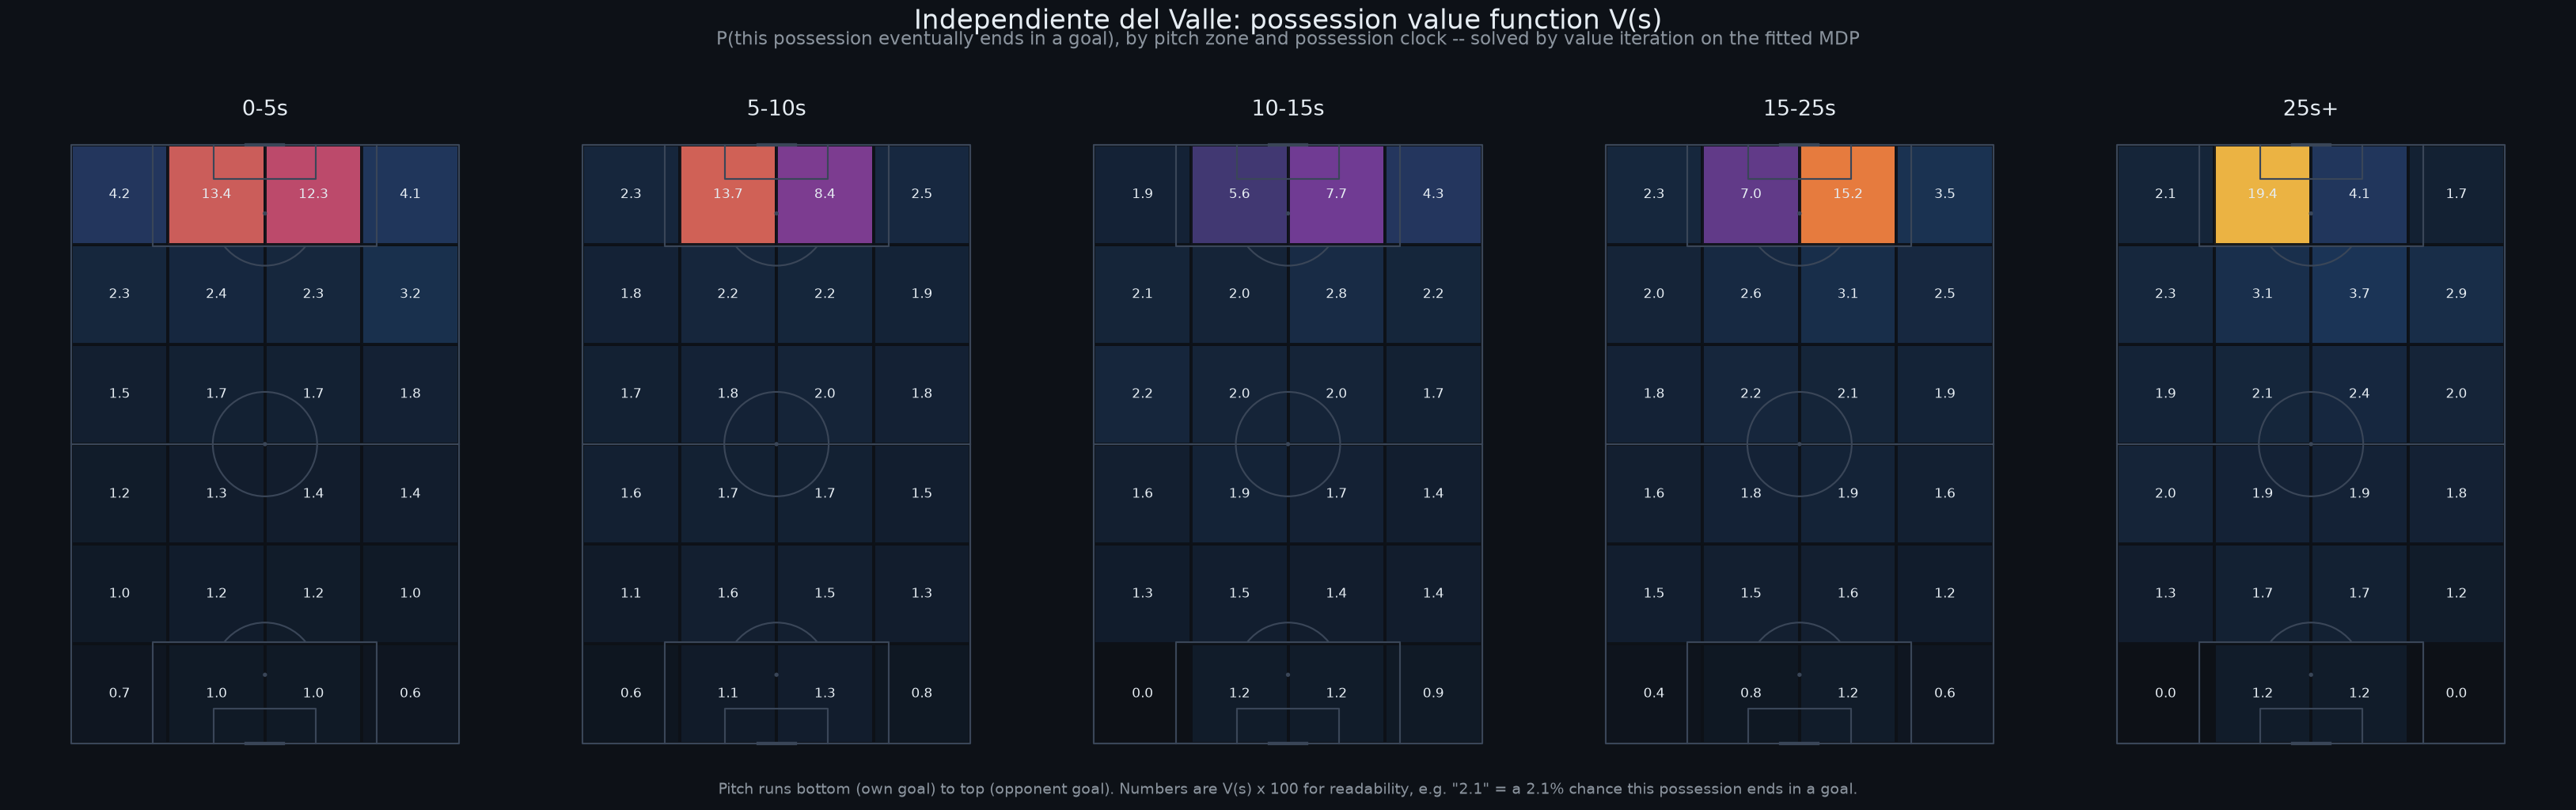
\includegraphics[width=\textwidth]{value_function_independiente_del_valle.png}
\caption{Solved value function $V(s)$ for Independiente del Valle: probability that a possession beginning in each pitch zone, at each possession-clock bucket, eventually ends in a goal. Value increases smoothly toward the opponent's goal in every clock bucket.}
\label{fig:valuefunction}
\end{figure}

\section{The Possession Simulator}
\label{sec:simulator}

The simulator draws whole possessions forward from the fitted MDPs while propagating parameter uncertainty. For each state-action pair, a transition vector is drawn once per simulated ``world,''
\begin{equation}
\tilde P(\cdot \mid s,a) \sim \Dir\big(\alpha_T(s,a)\big),
\end{equation}
using the team-average posterior parameters of Section~\ref{sec:teamavg} (or the lineup-level posterior for lineup-specific analysis). This single draw defines one internally consistent possible world for how the team's possessions behave. Episodes are then rolled out from an empirical distribution over possession-start zones: at each state, an action is sampled from the policy $\pi(a\mid s)$, the next state is sampled from the drawn $\tilde P(\cdot \mid s,a)$, and the possession clock advances, until the episode reaches $\GOAL$, $\NOGOAL$, or a maximum-length censor. Repeating this across many posterior draws and many rollouts per draw means the spread across draws -- not only the Monte Carlo noise within a draw -- reflects genuine parameter uncertainty in the fitted MDP.

The simulator deliberately separates the \emph{policy} $\pi(a\mid s)$, how often a team attempts each action type from a given state, from the \emph{dynamics} $P(s'\mid s,a)$ fit in Sections~\ref{sec:hierarchy}--\ref{sec:teamavg}, which describe how the world responds once a decision is attempted. This split is what makes altered-policy simulation meaningful (Section~\ref{sec:policy-sim}): we can reweight $\pi$ to ask ``what happens if this team attempts more crosses and fewer sideways passes'' while leaving the fitted execution quality of every decision exactly as observed.

\section{Empirical Results}
\label{sec:results}

We report five qualitative findings from fitting the model to the full Liga Pro season, each illustrating a different piece of the framework.

\subsection{Possession-clock nonstationarity}
\label{sec:results-hazard}

Figure~\ref{fig:hazard} shows, league-wide, the share of on-ball actions that continue the possession, end it in a turnover, end it in a saved or missed shot, or end it in a goal, as a function of the possession-clock bucket. Turnover risk is \emph{highest in the first five seconds} after a team wins the ball (22.9\%) and then falls and stabilizes around 16--17\% for the remainder of the possession -- the opposite of the shape a direct shot-clock analogy would predict, in which risk should rise as the clock runs out and the defense has more time to organize. A plausible reading is that turnovers spike immediately after a recovery because the ball is often still loosely contested or under first-touch pressure, and fall once the team has had a moment to organize possession. Figure~\ref{fig:teamhazard} disaggregates this by team: while most teams share the league-wide early spike, they differ substantially in level and in how much risk falls -- Manta FC, Macar\'a, and Mushuc Runa SC remain comparatively fragile late in a possession, while Aucas, Guayaquil City FC, and Cuenca are markedly steadier.

\begin{figure}[htbp]
\centering
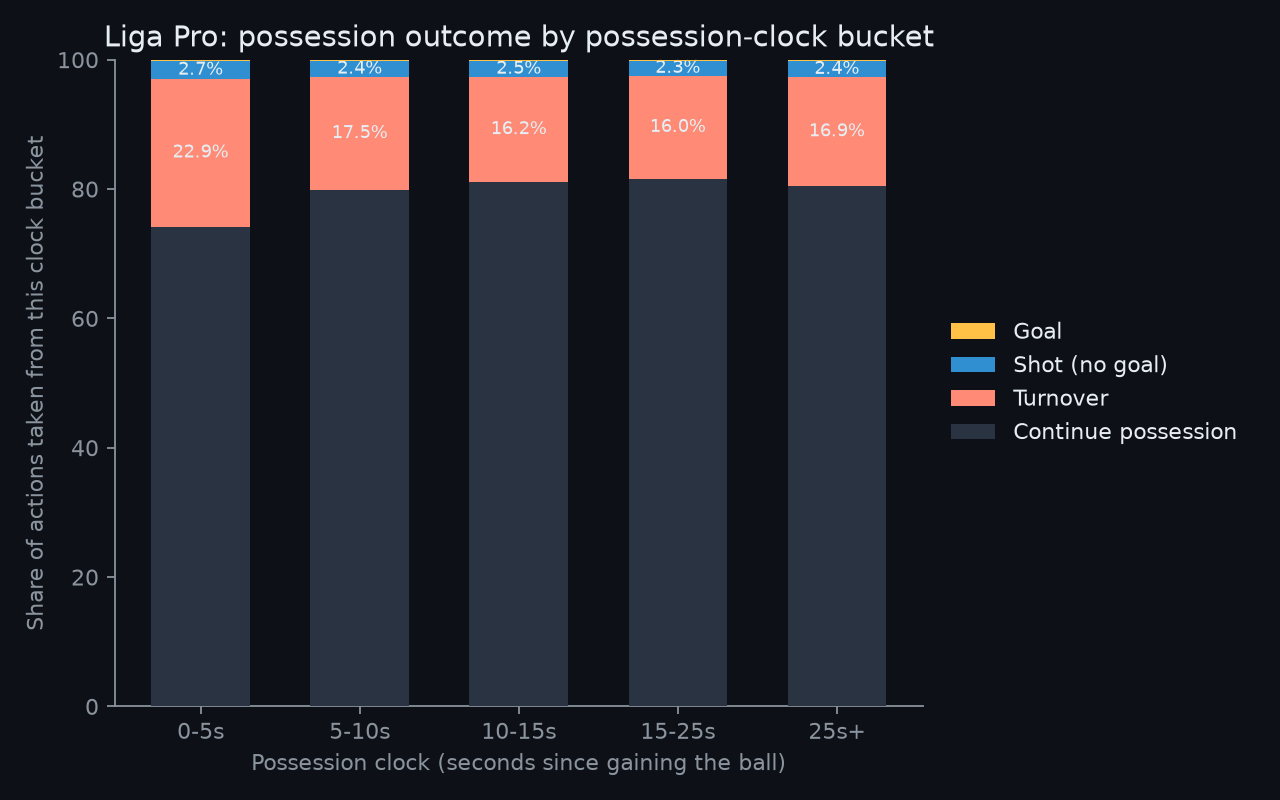
\includegraphics[width=0.85\textwidth]{possession_clock_hazard.png}
\caption{League-wide possession outcome by possession-clock bucket. Turnover risk peaks immediately after winning the ball rather than as the clock runs out.}
\label{fig:hazard}
\end{figure}

\begin{figure}[htbp]
\centering
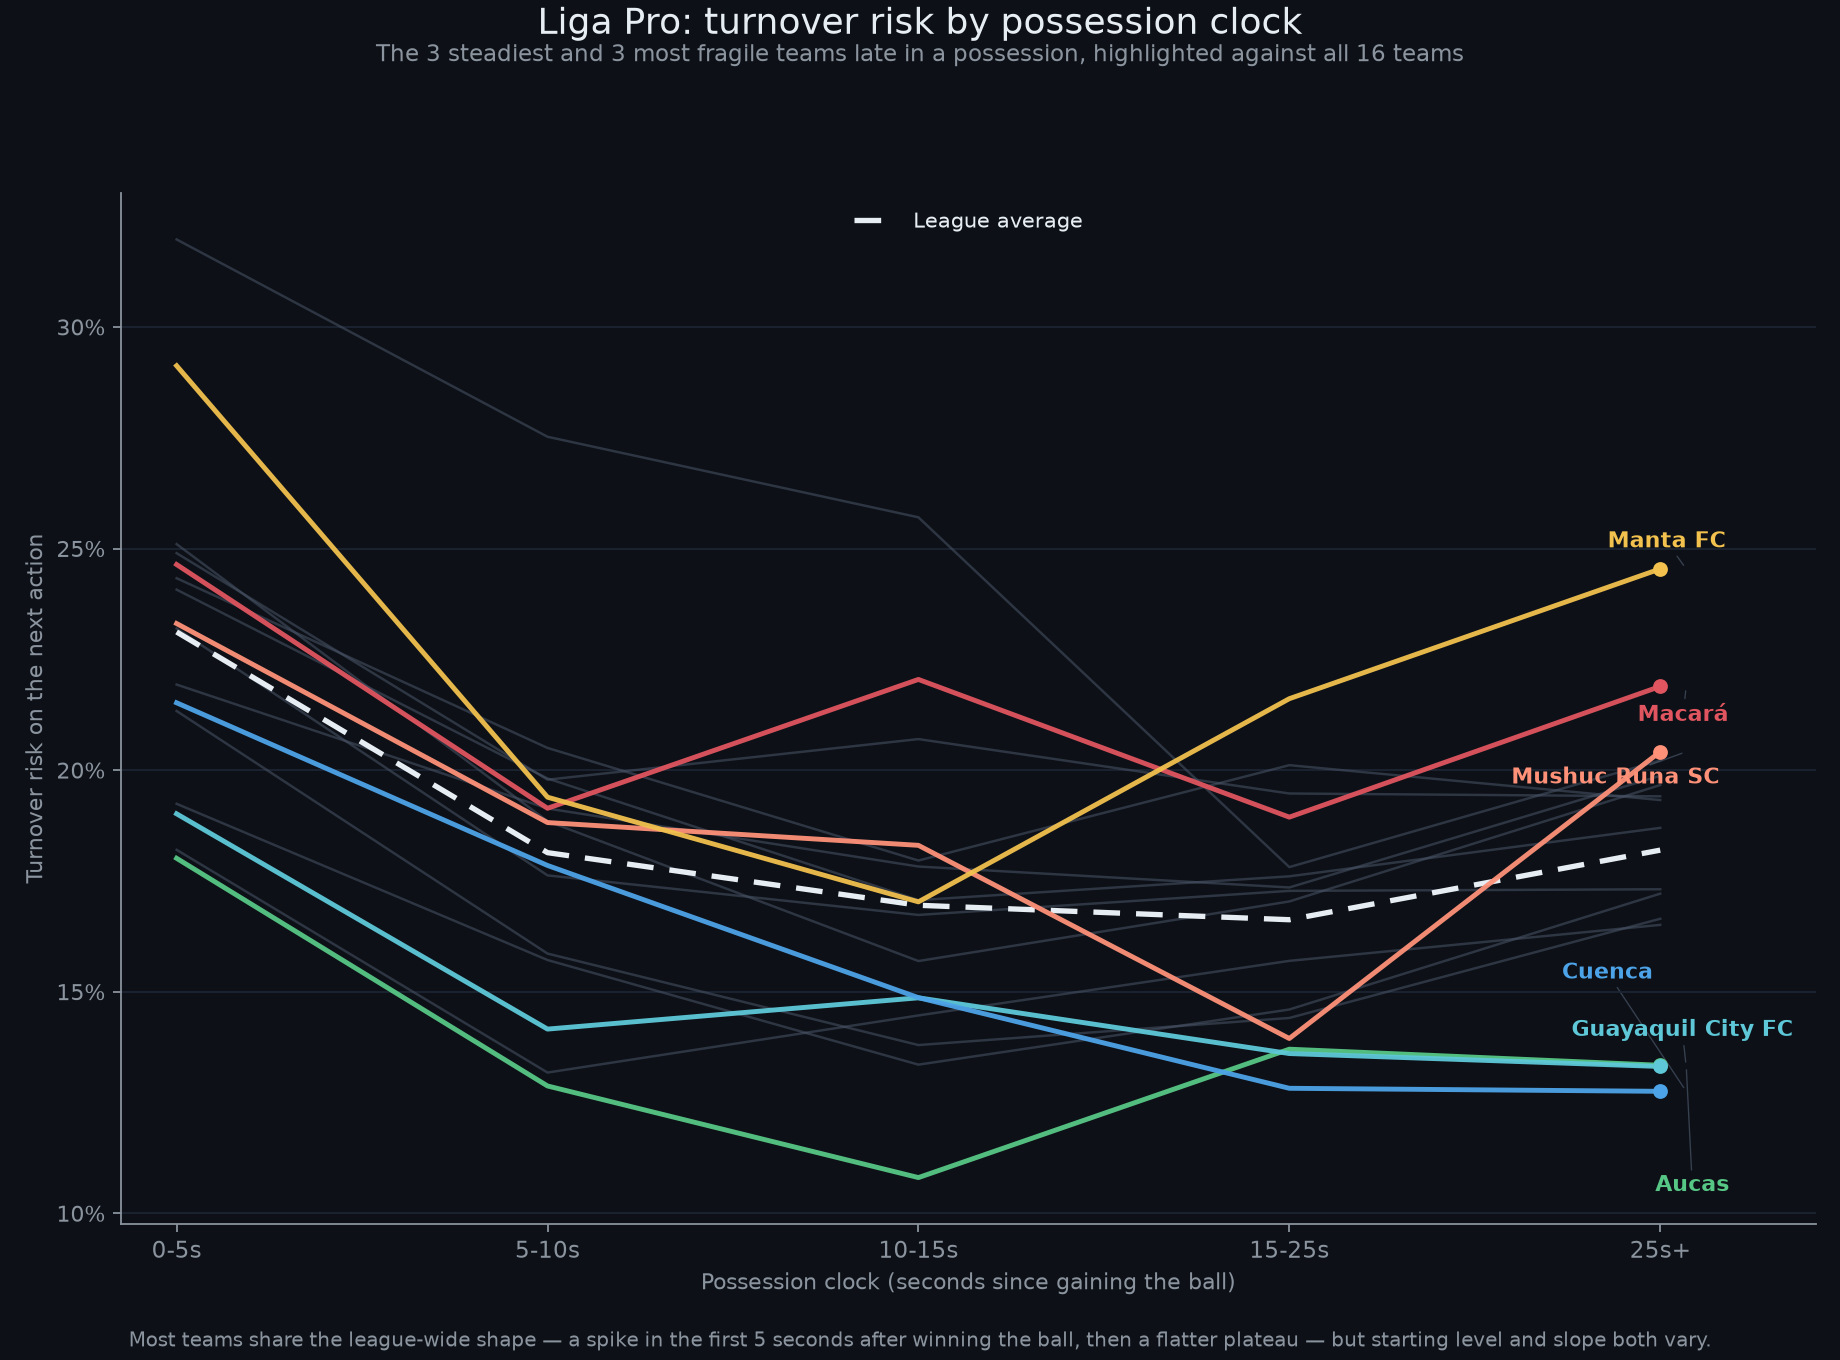
\includegraphics[width=0.85\textwidth]{team_clock_hazard.png}
\caption{Turnover risk by possession clock, per team, with the three steadiest and three most fragile teams highlighted against the league.}
\label{fig:teamhazard}
\end{figure}

\subsection{Zone value and shot generation}

Figure~\ref{fig:zoneheatmaps} shows shot-attempt rate and goal-conversion rate by pitch zone, league-wide, with zones supported by fewer than 15 shots masked rather than reported (several defensive-third zones have a handful of shot attempts -- some the residue of blocked clearances -- for which a raw conversion rate would be pure noise; we mask rather than report these, in the same spirit as the own-goal exclusion of Section~\ref{sec:data}). Shot-attempt rate is concentrated almost entirely in the attacking third, peaking at 46--50\% of visits to the central zones directly in front of goal; goal-conversion rate given a shot follows the same gradient, from roughly 4--5\% in wide attacking areas to 13--14\% centrally in the box. This is consistent with, and reproduced independently by, the value function of Section~\ref{sec:valuefunction}.

\begin{figure}[htbp]
\centering
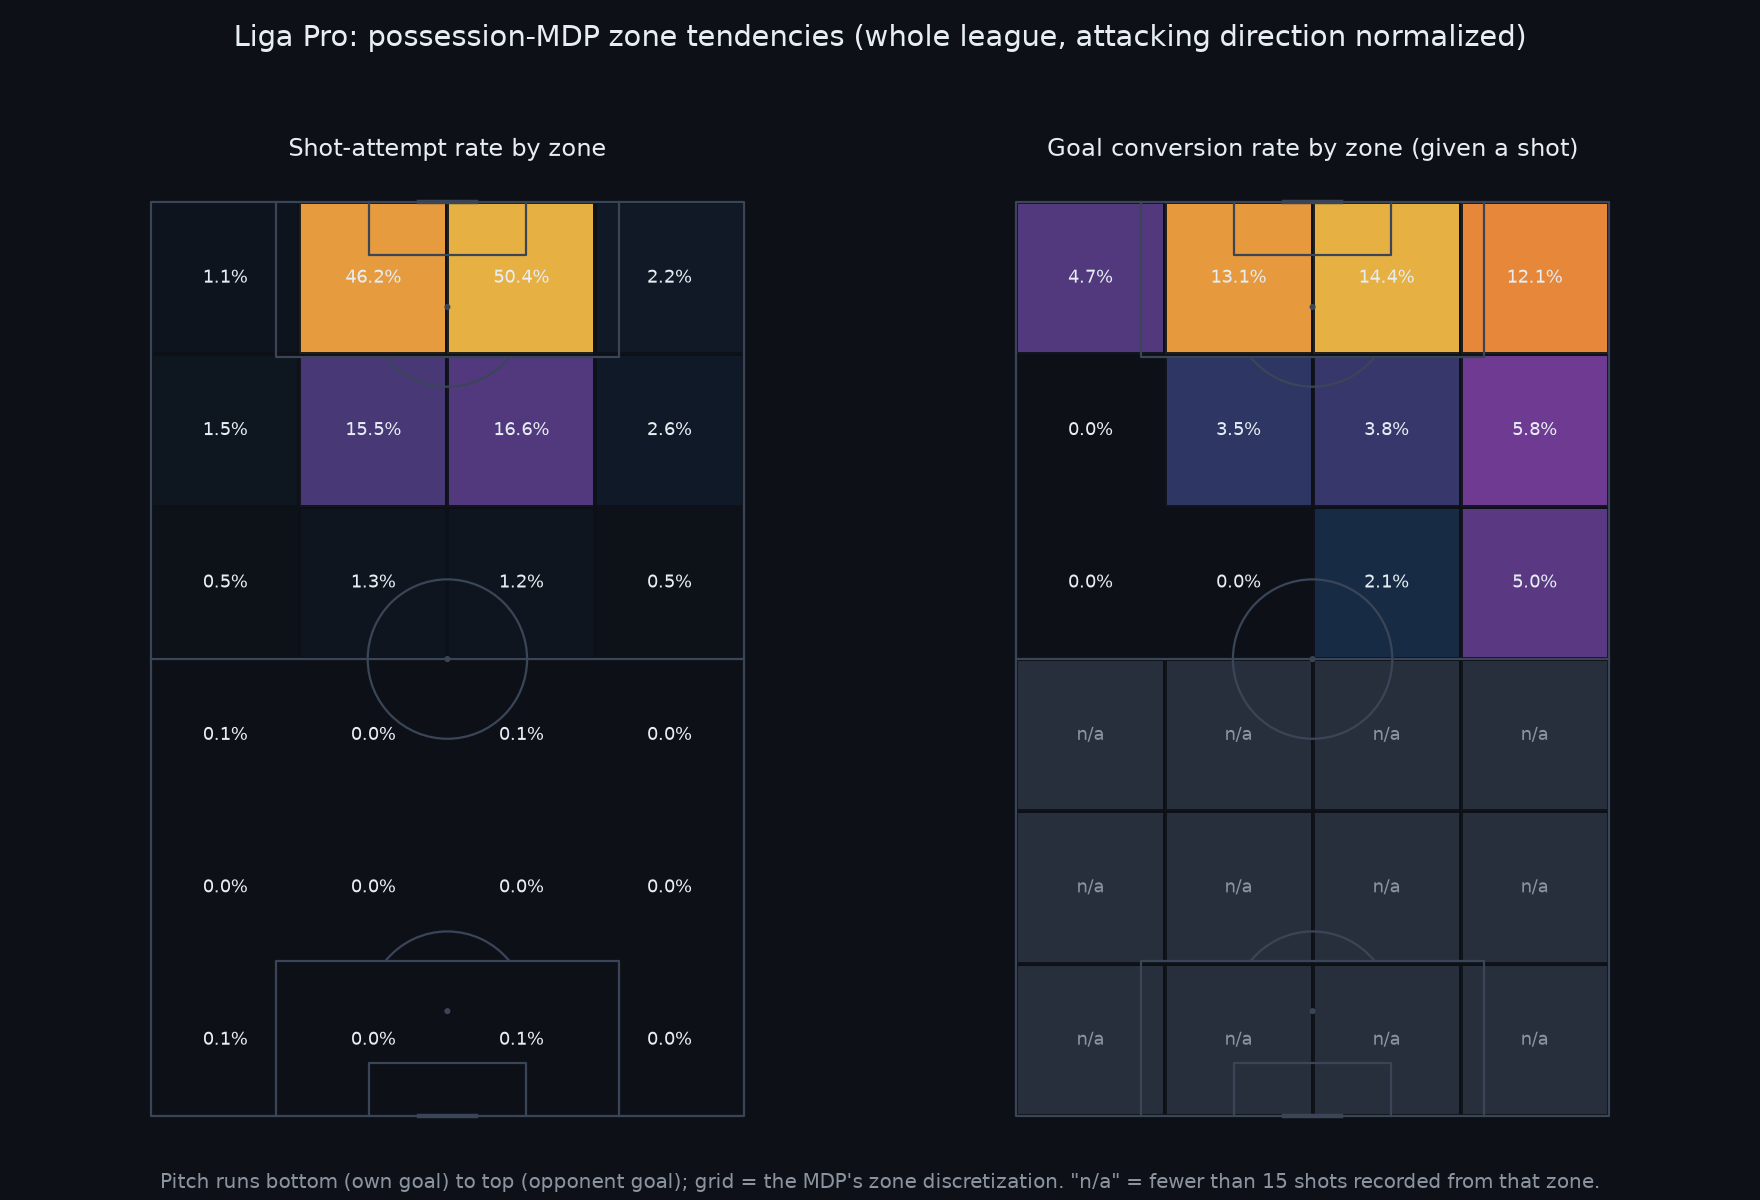
\includegraphics[width=0.85\textwidth]{zone_heatmaps.png}
\caption{League-wide shot-attempt rate and goal-conversion rate by pitch zone. Zones with fewer than 15 shots are masked (``n/a'') rather than reported.}
\label{fig:zoneheatmaps}
\end{figure}

\subsection{Team build-up style}

The fitted policy also characterizes each team's revealed build-up \emph{style}: the marginal, visit-weighted mix of forward (advance $+$ cross), sideways, and backward actions, excluding the rare shot decision, which we visualize as a ternary plot (Figure~\ref{fig:ternary}). Because these three shares are comparably sized (forward 35--47\%, sideways 43--52\%, backward 11--18\% across the league), teams spread across a genuine region of the simplex rather than collapsing toward one corner, unlike the $\{\GOAL, \NOGOAL, \TURN\}$ outcome split, which is turnover-dominated for every team and would crowd all 16 points into a single corner of the same diagram. Marker size encodes each team's simulated on-policy goal rate per possession (Section~\ref{sec:policy-sim}); notably, Independiente del Valle's goal rate is the league's highest despite an unremarkable build-up-style position, consistent with the model attributing their attacking output to execution quality (the fitted dynamics) rather than to an unusual style (the fitted policy).

\begin{figure}[htbp]
\centering
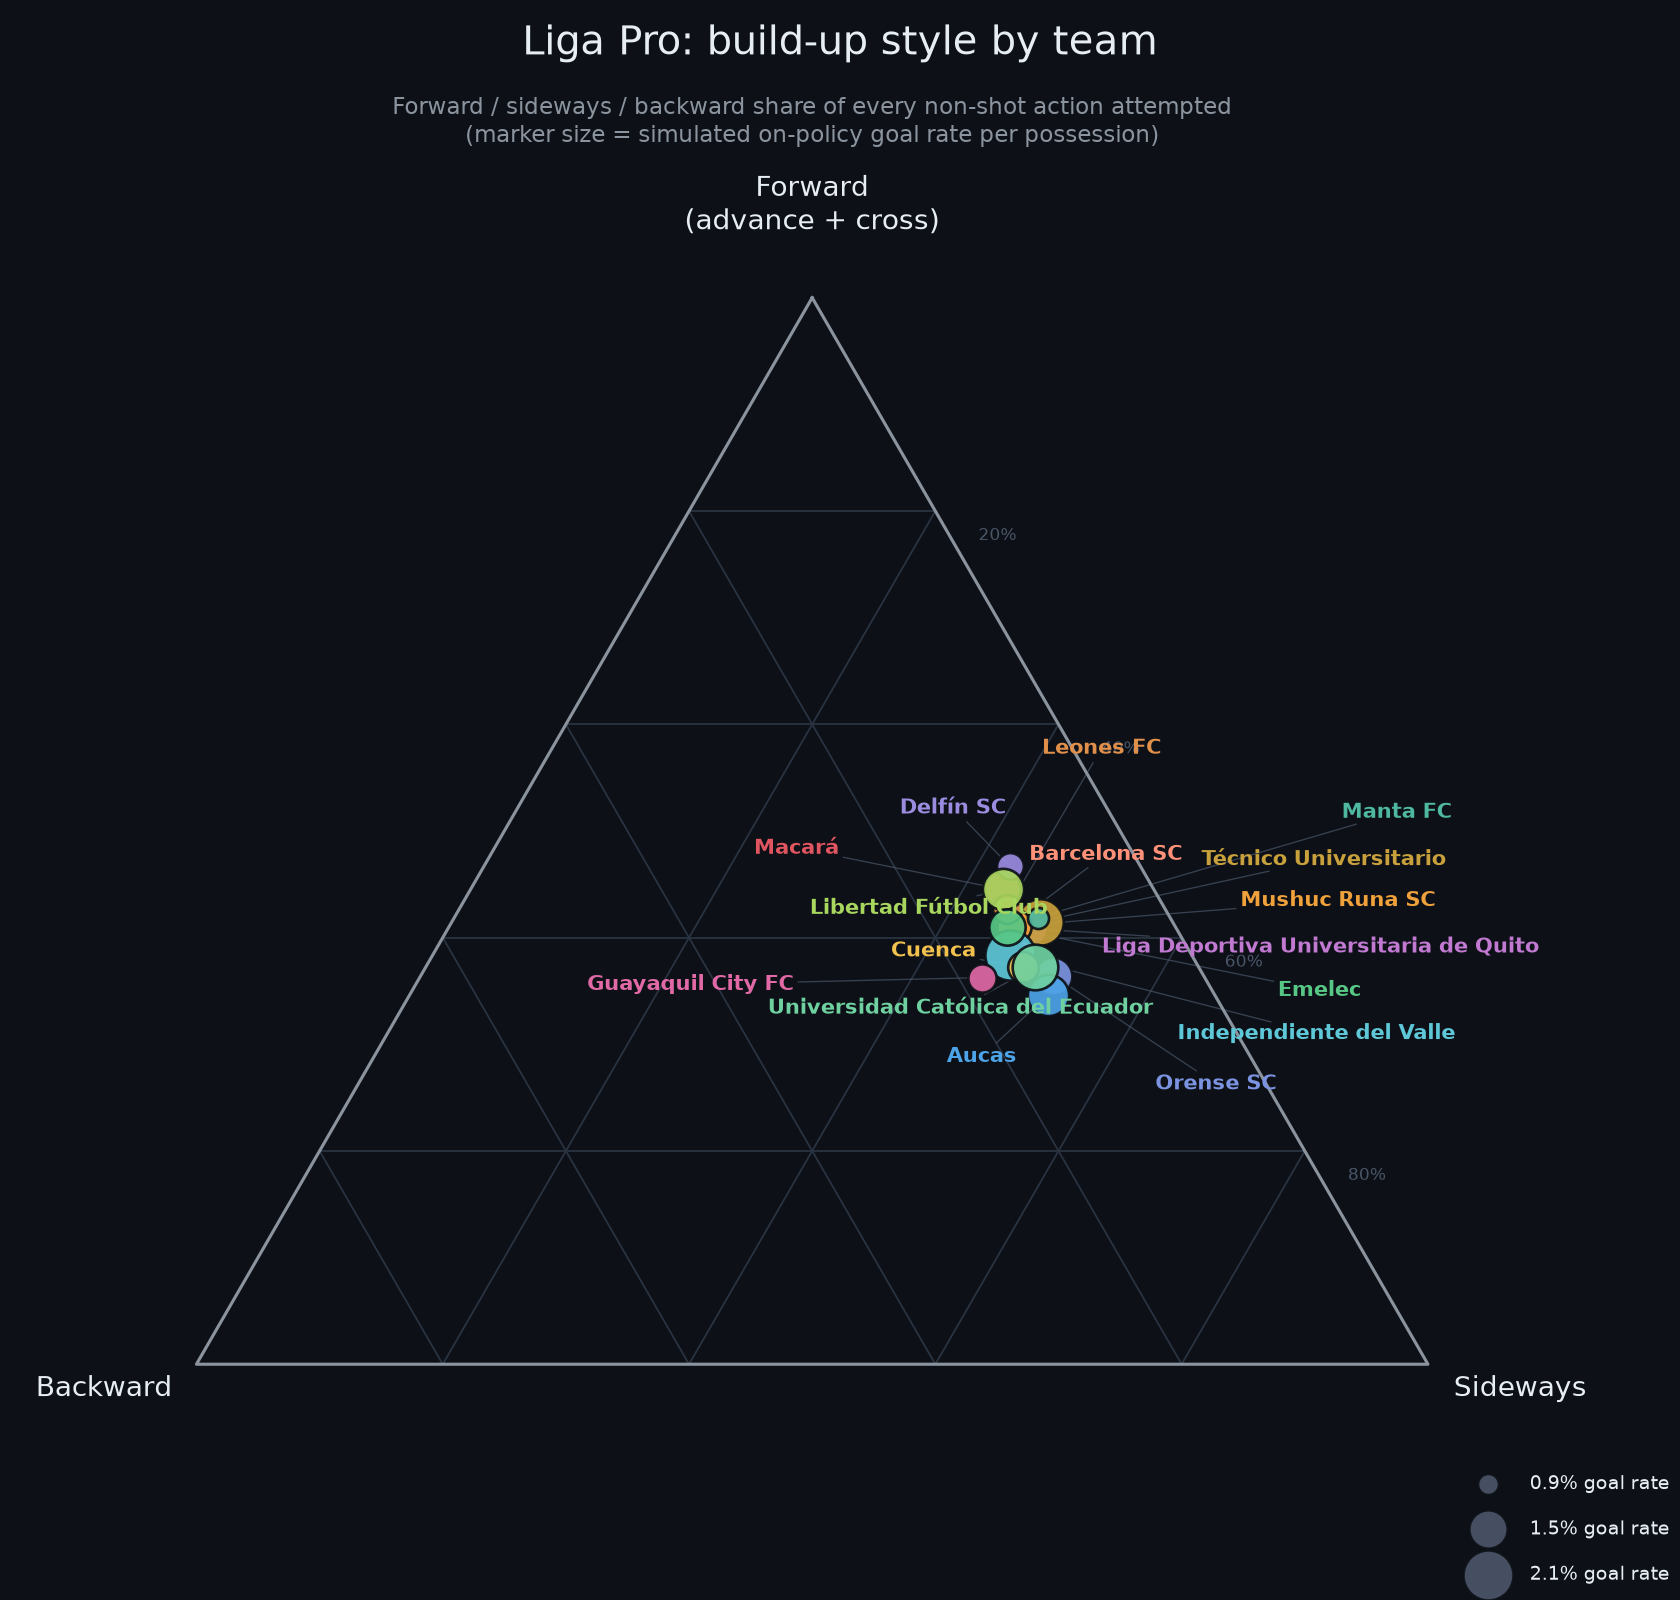
\includegraphics[width=0.72\textwidth]{team_style_ternary.png}
\caption{Forward/sideways/backward share of every non-shot action attempted, by team; marker size is simulated on-policy goal rate per possession.}
\label{fig:ternary}
\end{figure}

\subsection{Season form}

Because possession episodes carry match dates, the same shot-ending-rate-per-possession statistic can be tracked match by match. Figure~\ref{fig:formtrend} shows a five-match rolling average for every team, ordered by current form. The trends are not uniform in shape: Independiente del Valle opens the season at the league's highest rate ($\sim$21\%) and trends down to $\sim$15\%, while Liga Deportiva Universitaria de Quito rises from the bottom of the league ($\sim$6\%) to among the highest ($\sim$15\%) by the same point in the season -- a reminder that a single-season average, as reported elsewhere in this section, can obscure materially different in-season trajectories.

\begin{figure}[htbp]
\centering
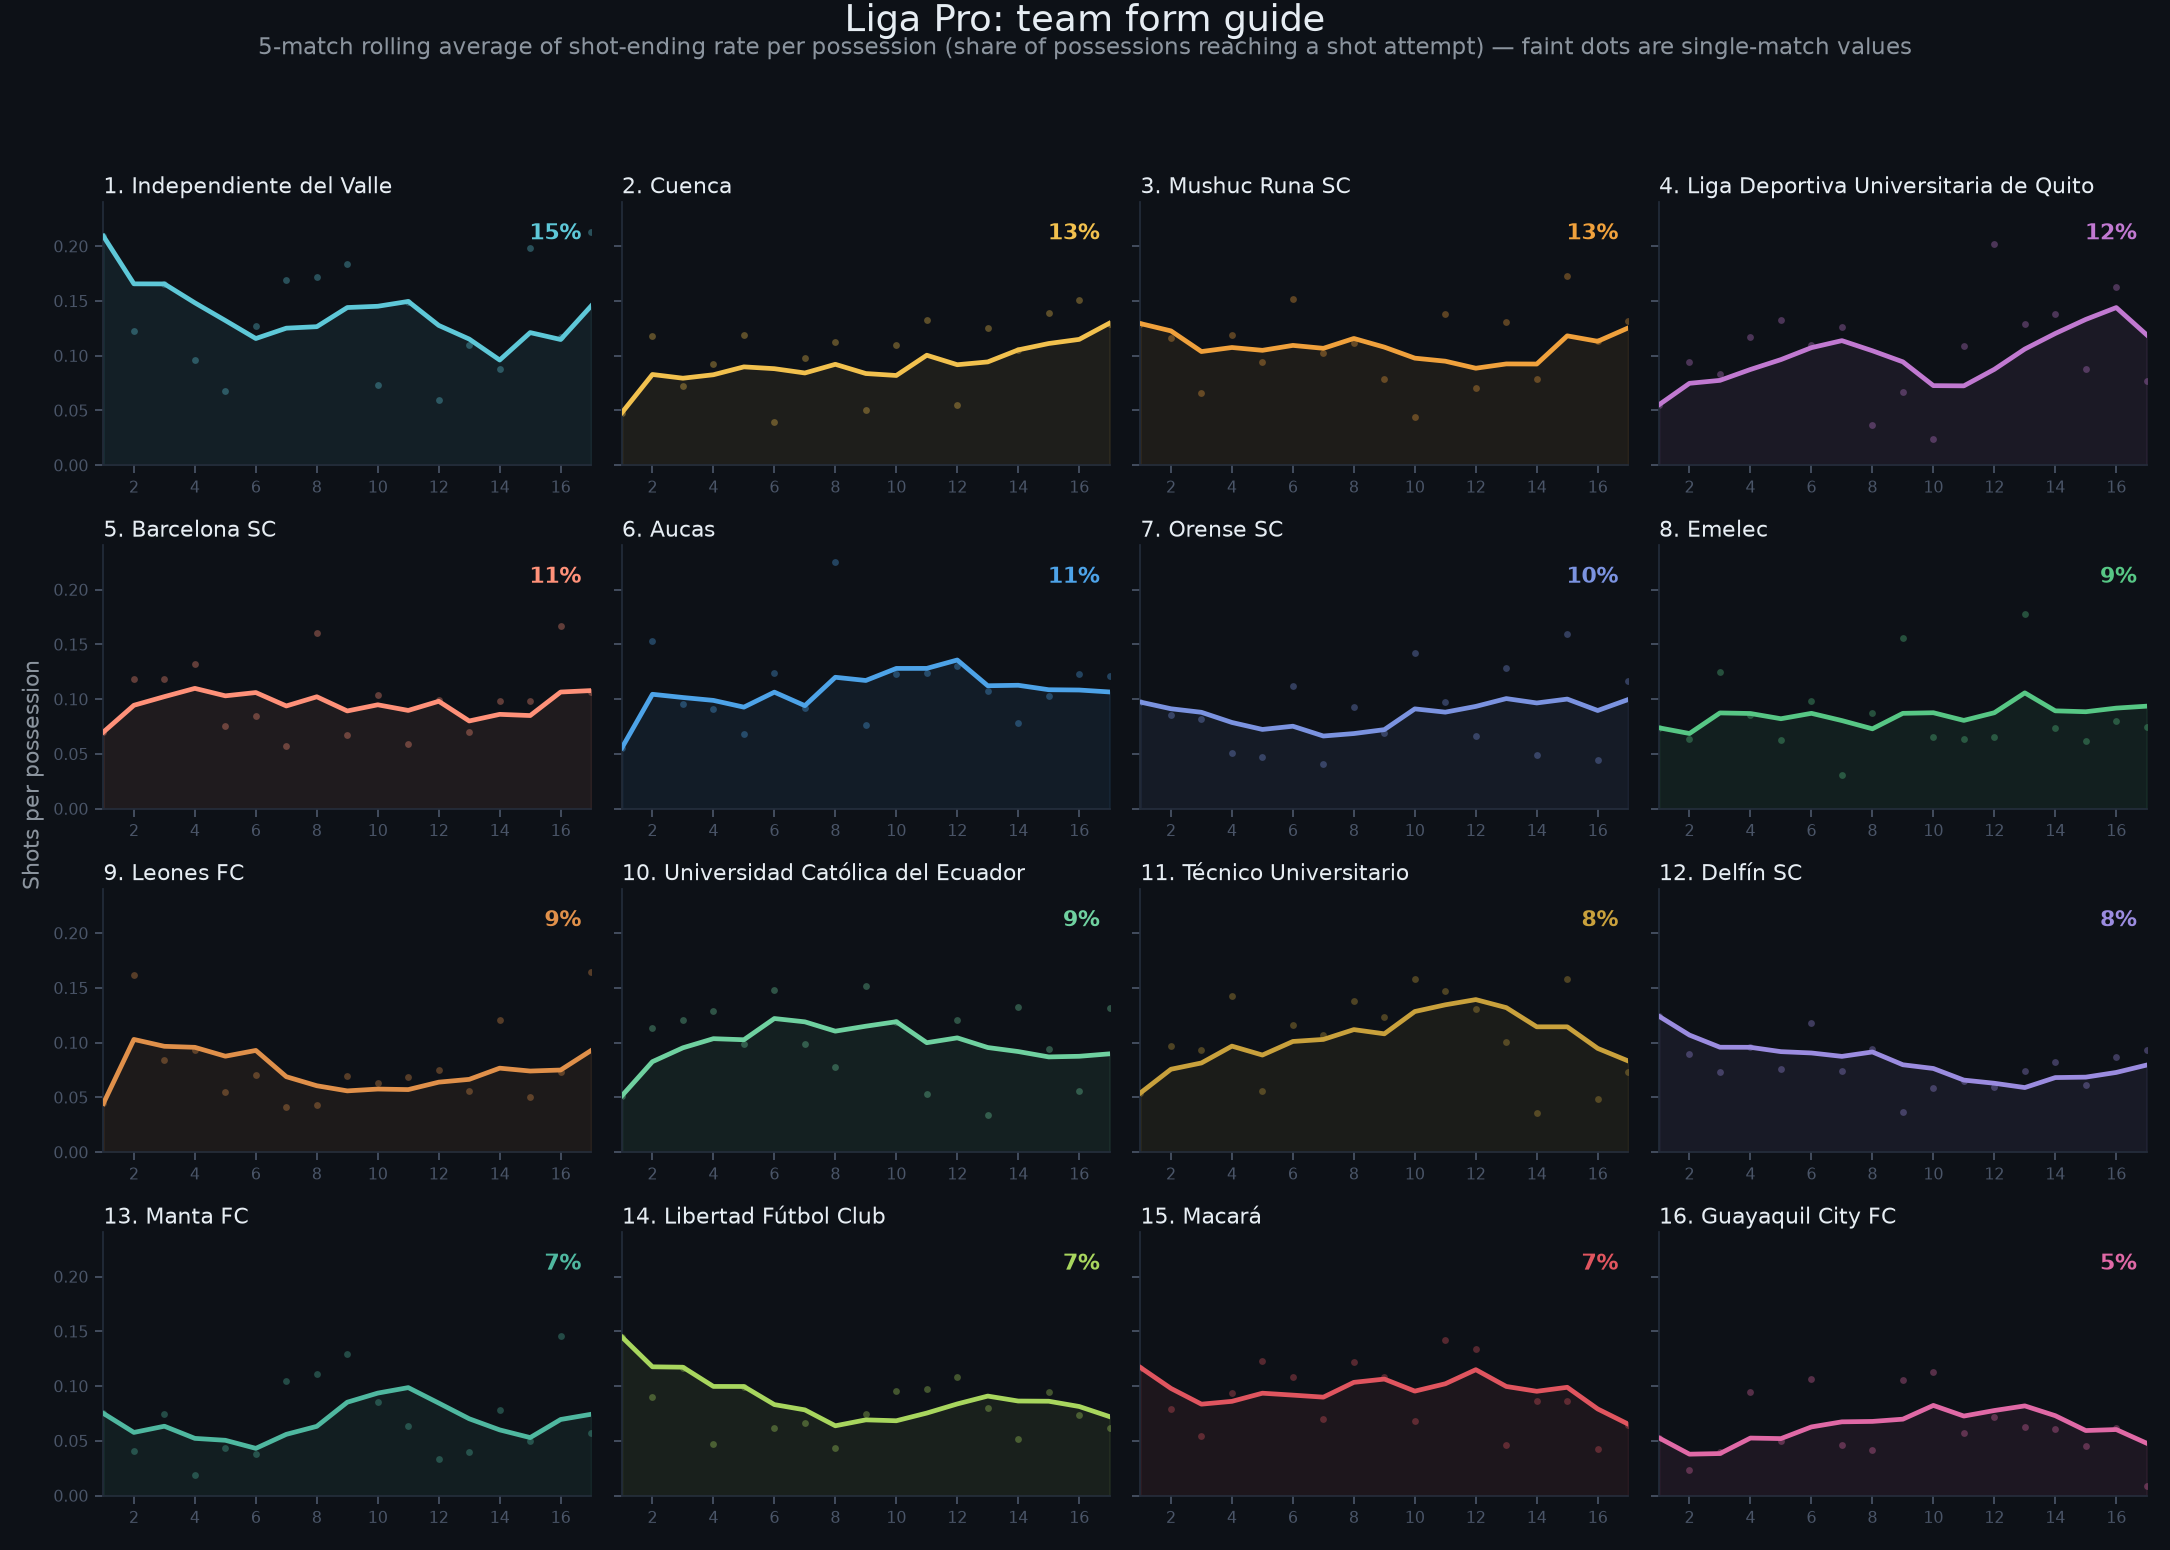
\includegraphics[width=\textwidth]{team_form_trend.png}
\caption{Five-match rolling average of shot-ending rate per possession, all 16 teams, ranked by current form. Faint points are single-match values.}
\label{fig:formtrend}
\end{figure}

\subsection{League ranking}

Figure~\ref{fig:leaguecomparison} ranks all 16 teams by simulated on-policy goal rate per possession, with 95\% predictive intervals from the posterior-draw simulation of Section~\ref{sec:simulator}. Independiente del Valle and Universidad Cat\'olica del Ecuador separate from the rest of the league (2.4\% and 2.0\% respectively); the remaining teams cluster between roughly 0.6\% and 1.6\% with overlapping intervals, indicating the model does not support fine-grained ranking distinctions among most of the league on this statistic alone.

\begin{figure}[htbp]
\centering
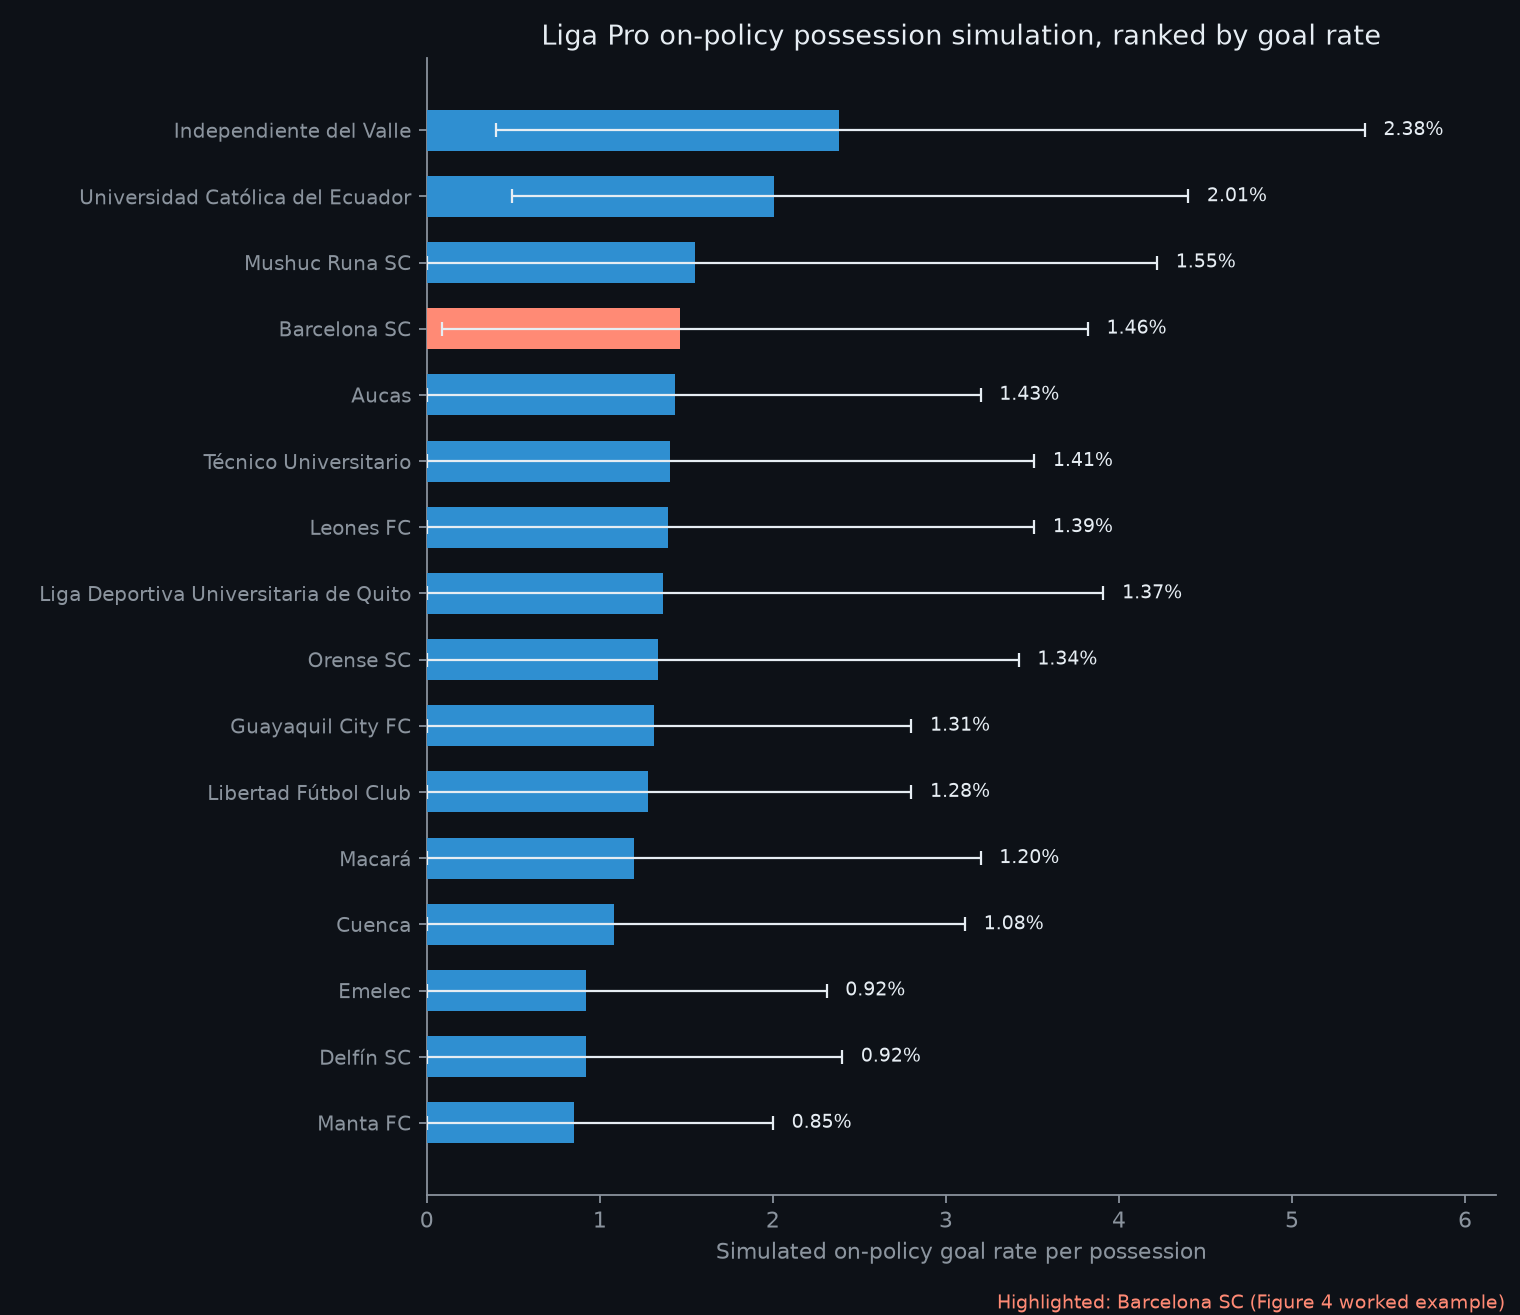
\includegraphics[width=0.85\textwidth]{league_team_comparison.png}
\caption{Simulated on-policy goal rate per possession, all 16 teams, with 95\% predictive intervals.}
\label{fig:leaguecomparison}
\end{figure}

\section{Policy Counterfactuals: On-Policy versus Altered-Policy Simulation}
\label{sec:policy-sim}

\subsection{An altered policy}

We define a mechanical ``directness'' policy alteration: in the middle and attacking thirds, probability mass shifts from the sideways/back actions to the advance/cross actions (a $+15$ percentage-point shift, renormalized), holding the fitted dynamics $P(s'\mid s,a)$ fixed. Figure~\ref{fig:actionmix} shows this concretely for one real, well-populated state (Independiente del Valle, final third, right touchline, 0--5s into the possession): under the on-policy distribution the team attempts sideways passes 39\% of the time and advances or crosses a combined 36\% of the time; under the altered policy these move to 33\% and 46\% respectively, while the shot decision (3\%) is untouched, since this particular alteration only reweights ball-circulation decisions.

\begin{figure}[htbp]
\centering
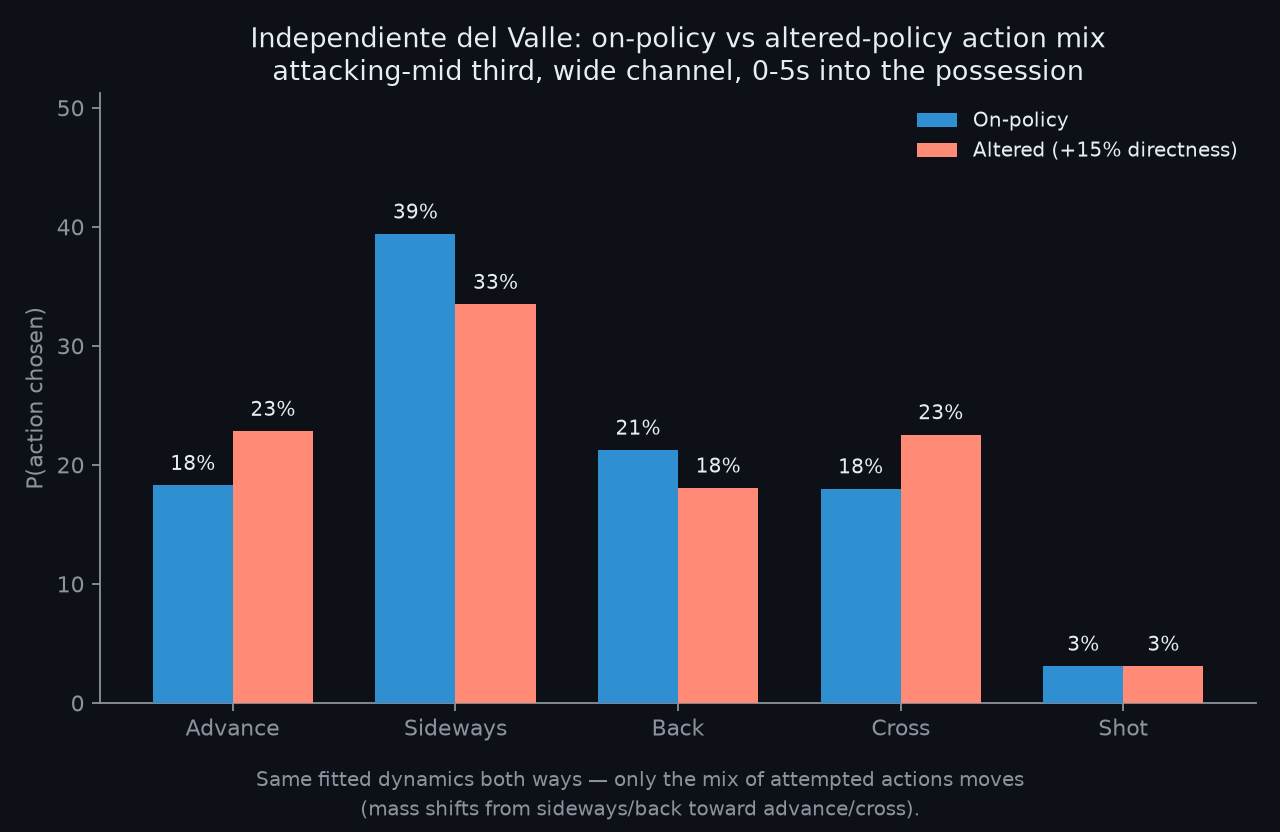
\includegraphics[width=0.72\textwidth]{policy_action_mix_independiente_del_valle.png}
\caption{On-policy vs.\ altered-policy action-choice probabilities for one real fitted state. Only the decision mix moves; the fitted dynamics are identical under both policies.}
\label{fig:actionmix}
\end{figure}

\subsection{Statistical reliability of the comparison}
\label{sec:pairing}

A first implementation of this comparison ran two independent calls to the simulator -- one under $\pi_{\text{on}}$, one under $\pi_{\text{altered}}$ -- and differenced their simulated goal rates. Because goal rate is a rare-event statistic (roughly 1--2\% per possession even for strong teams), and because each of the two calls draws its own independent posterior sample of the shared dynamics $P(s'\mid s,a)$, this estimator is considerably noisier than it appears: re-running the identical comparison with a different random seed changed Independiente del Valle's estimated effect from $+0.15$ percentage points to $-0.39$ percentage points, a sign flip driven entirely by Monte Carlo noise in two independently-drawn dynamics samples rather than by any real difference in the policies being compared.

We correct this with a paired design: within each simulated ``world,'' both $\pi_{\text{on}}$ and $\pi_{\text{altered}}$ are rolled out against the \emph{same} drawn dynamics sample $\tilde P(\cdot\mid s,a)$, so that only the policy difference -- not independently-redrawn execution quality -- drives the per-world difference in outcome. We further report the 95\% confidence interval of the \emph{mean} paired difference (via the normal approximation to the standard error of the mean across worlds) rather than the predictive spread of the raw per-world differences, since the latter conflates the (wide) uncertainty in any one simulated world with the (much narrower) uncertainty in the average effect the comparison is actually trying to estimate. Figure~\ref{fig:policycomparison} shows the resulting on-policy vs.\ altered-policy comparison for Independiente del Valle under this design.

\begin{figure}[htbp]
\centering
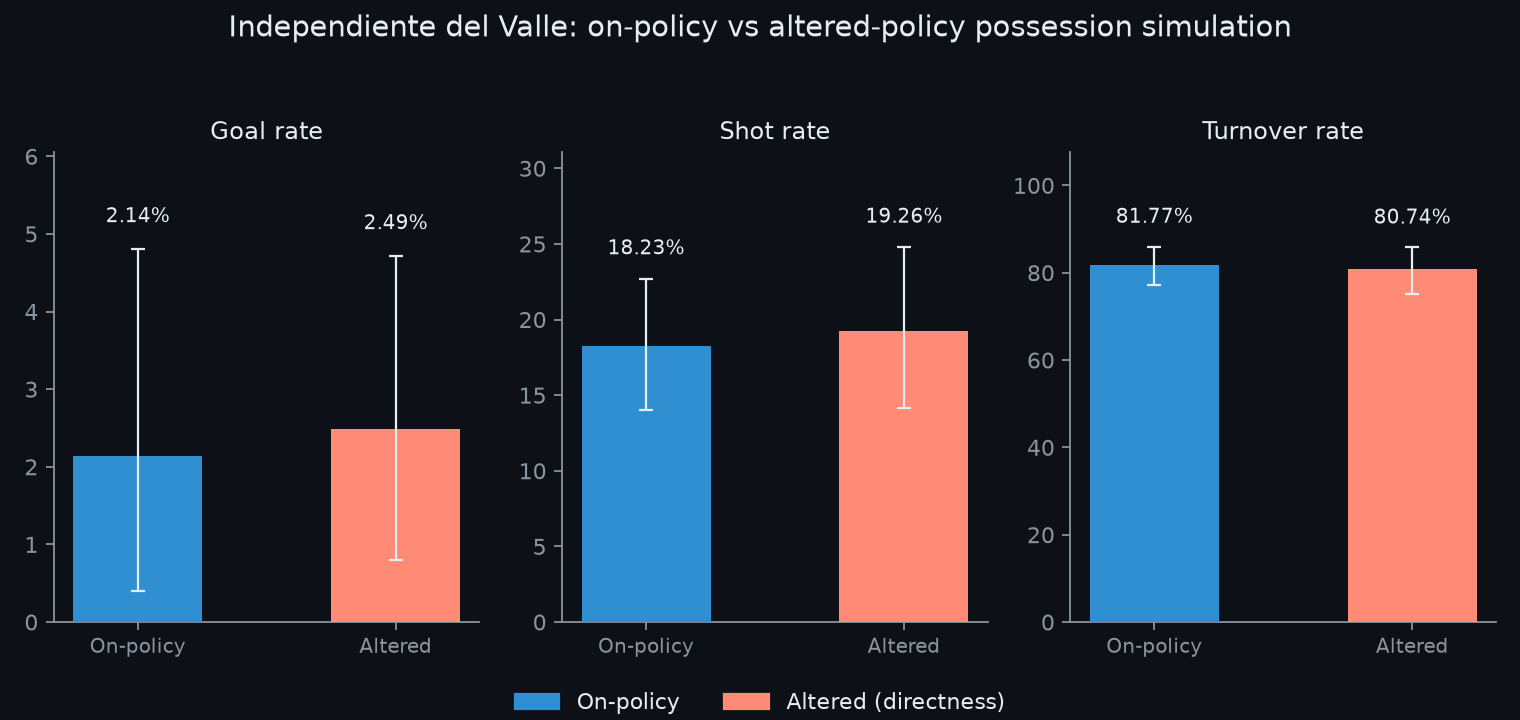
\includegraphics[width=0.85\textwidth]{policy_comparison_independiente_del_valle.png}
\caption{On-policy vs.\ altered-policy simulated possession outcomes for Independiente del Valle, with 95\% predictive intervals.}
\label{fig:policycomparison}
\end{figure}

\subsection{League-wide directness ranking}

Figure~\ref{fig:directness} ranks all 16 teams by the paired-simulation estimate of the directness policy's effect on simulated on-policy goal rate. Three teams -- Independiente del Valle ($+0.73$ pp, 95\% CI $+0.33$ to $+1.13$), Universidad Cat\'olica del Ecuador ($+0.48$ pp, CI $+0.12$ to $+0.84$), and Orense SC ($+0.43$ pp, CI $+0.08$ to $+0.78$) -- show an effect whose confidence interval excludes zero. For the remaining 13 teams the interval straddles zero: the model does not support a confident claim that the altered policy helps or hurts, which is the correct conclusion to draw given the modest size of the policy perturbation and the rarity of the outcome being measured, not a failure of the method.

\begin{figure}[htbp]
\centering
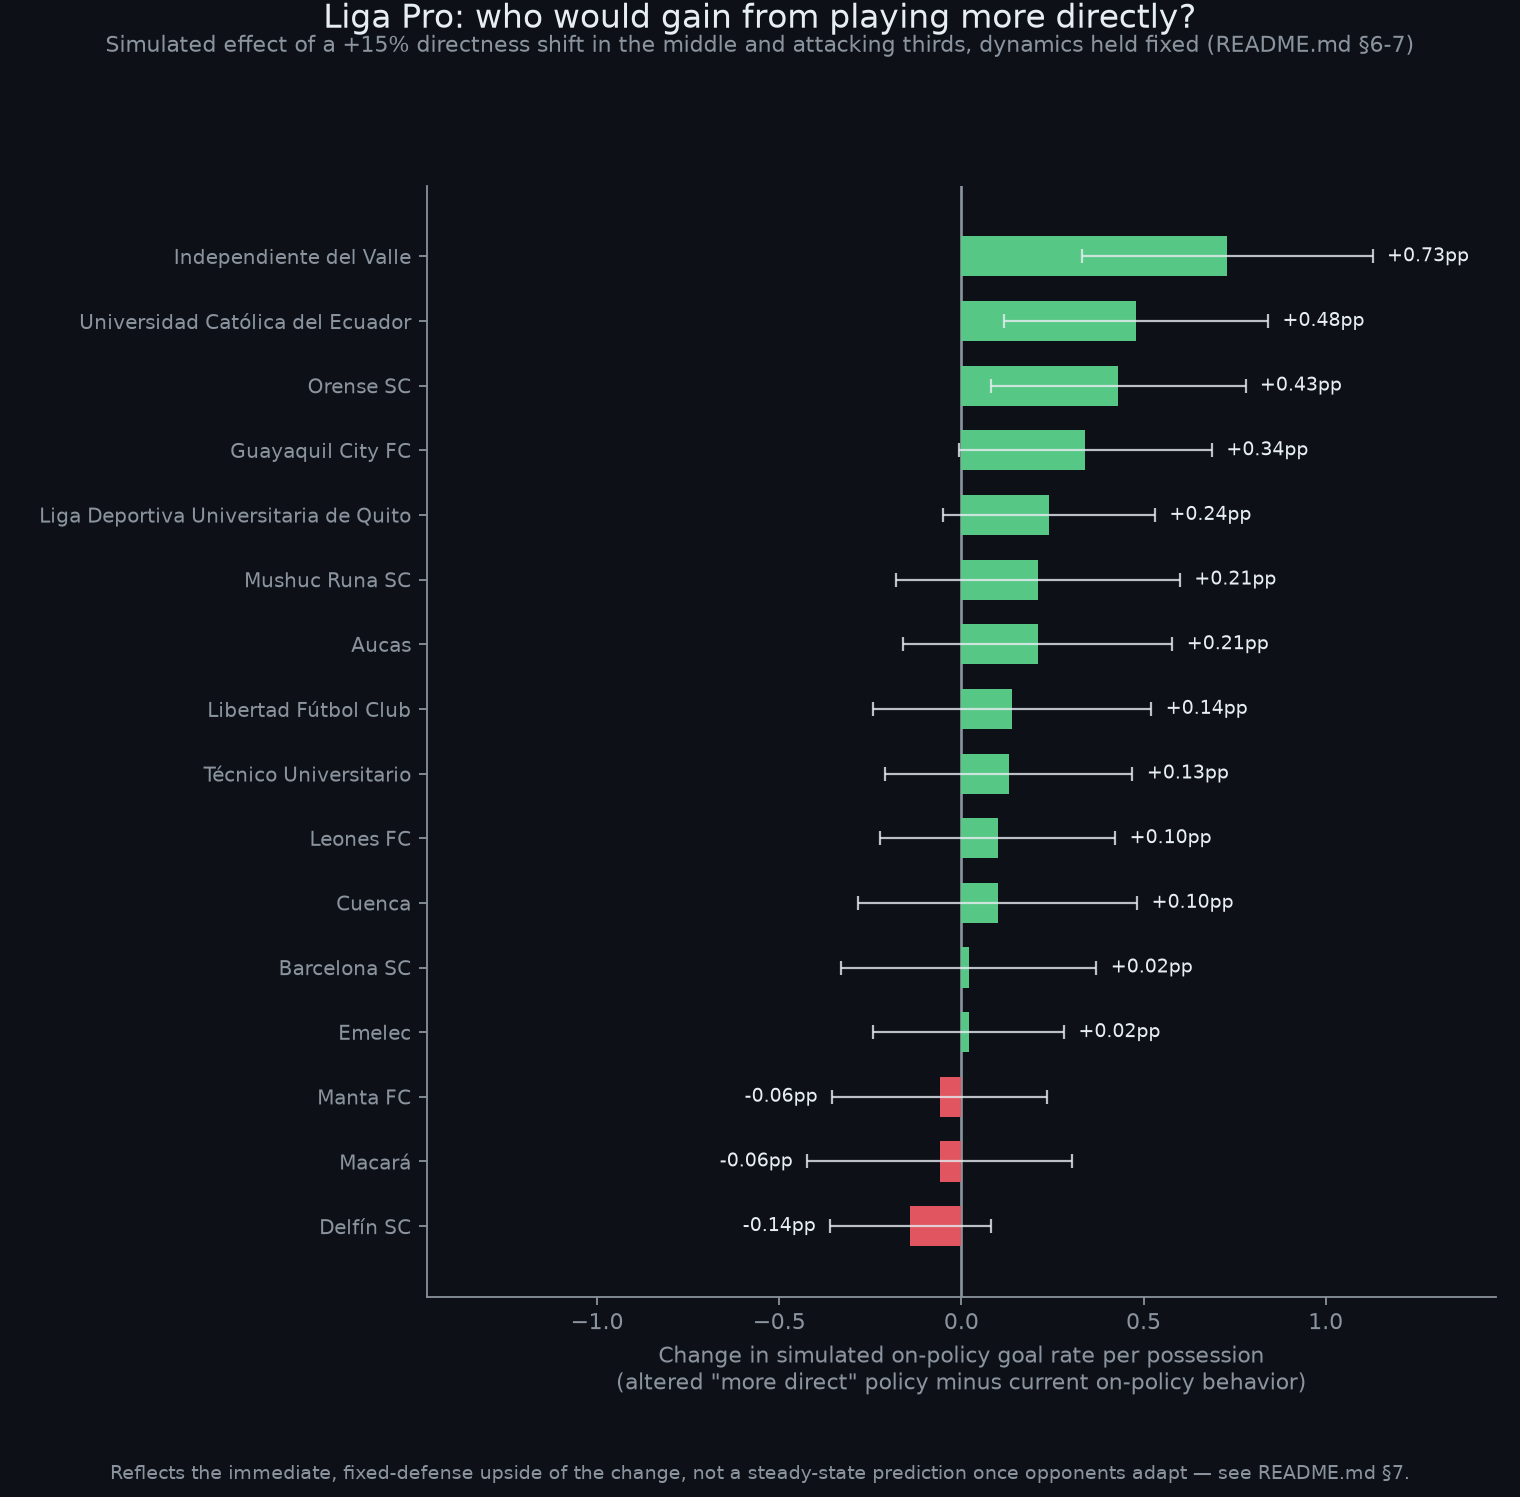
\includegraphics[width=0.85\textwidth]{directness_ranking.png}
\caption{Change in simulated on-policy goal rate under the altered (``more direct'') policy, all 16 teams, with 95\% confidence intervals of the mean paired effect.}
\label{fig:directness}
\end{figure}

\section{Game-Theoretic Considerations}
\label{sec:gametheory}

The transition probabilities $P(s'\mid s,a)$ fit in Sections~\ref{sec:hierarchy}--\ref{sec:teamavg} are not policy-invariant: they were generated by defenses reacting to a team's \emph{actual}, observed tendencies. If a team rarely crosses from deep wide positions, opposing full-backs need not respect that threat and can squeeze infield, which is part of why the fitted completion and turnover rates for crossing look the way they do in the data. Simulating an altered policy while holding $P(s'\mid s,a)$ fixed therefore implicitly assumes the opponent's defensive shape does not change in response -- a reasonable first-order approximation for a small, one-off deviation, but increasingly wrong the larger and more sustained the shift, and wrong in a predictable direction: a defense that adapts should suppress exactly the transitions a sustained policy change tries to exploit, so the fixed-dynamics estimates of Section~\ref{sec:policy-sim} are better read as an upper bound on the immediate, surprise-value benefit of a change than as a steady-state prediction. This argues for validating any promising altered policy in short, in-season bursts before adopting it as a full-match identity, and for treating the ``correct'' policy as a best response in a game between two teams' policies -- an equilibrium concept -- rather than a single-agent optimization over a fixed opponent. Extending the simulator to iterate policy adjustments against a simulated opponent response (a fictitious-play loop over the fitted MDPs) is the natural next step, left for future work.

\section{Limitations and Future Work}
\label{sec:limitations}

The zone/clock/action discretization is coarse by design; finer grids would need materially more matches of data per lineup before hierarchical shrinkage stops dominating the lineup-level estimates. Set pieces (corners, free kicks, throw-ins) are folded into the general turnover/restart handling rather than modeled as their own sub-MDPs with set-piece-specific routines. The Markov assumption of Section~\ref{sec:markov} means the model cannot represent history-dependent effects such as fatigue, momentum, or game-state (scoreline) effects on decision-making, all of which are plausible drivers of real transition probabilities that the current state representation does not capture. The game-theoretic discussion of Section~\ref{sec:gametheory} is qualitative; no opponent-adaptation term is fit into the model, and the paired-simulation correction of Section~\ref{sec:pairing}, while it resolves the sign-flip instability we observed, still inherits whatever bias the fixed-dynamics assumption itself introduces for large policy perturbations.

\section{Conclusion}

We have adapted a shot-clock-dependent basketball possession-MDP framework to football, replacing the shot clock with an endogenous possession clock, and shown that the resulting model is fittable to a single season of league event data via a three-level Bayesian hierarchy and a lineup-to-team-average transition-weighting scheme with a provable expected-count consistency property. The fitted model's value function, possession-clock hazard curves, and build-up-style geometry all produce qualitatively sensible, non-trivial results, and its explicit separation of policy from dynamics supports counterfactual policy simulation -- provided that rare-event comparisons are estimated with a paired design, which we show is necessary rather than optional. The game-theoretic caveat of Section~\ref{sec:gametheory} bounds how far any single-agent counterfactual simulation of this kind can be trusted, and motivates the natural next step of an opponent-adaptive extension.

\section*{Software and Reproducibility}
The complete implementation -- possession segmentation, hierarchical model fitting, the team-average weighting scheme, the Monte Carlo simulator, value iteration, and every figure in this paper -- is available in the \texttt{PossessionMDP/} directory of this project's repository, along with the underlying Opta-style event data for the season analyzed.

\bibliographystyle{apalike}
\begin{thebibliography}{1}

\bibitem[Cervone et al.(2016)]{cervone2016multiresolution}
Cervone, D., D'Amour, A., Bornn, L., and Goldsberry, K. (2016).
\newblock A multiresolution stochastic process model for predicting basketball possession outcomes.
\newblock \emph{Journal of the American Statistical Association}, 111(514).
\newblock \doi{10.1080/01621459.2016.1141685}.

\end{thebibliography}

\end{document}
